\section{Whitening-based Computing $\BLap(\Phi)$}

In this section, we propose an algorithm to compute approximate set of backbone literals $\BLap(\Phi)$, namely Whiten-based Algorithm. As mentioned in Section \ref{sec:overview}, finding more backbone at the earlier stage of the computing provides benefits for the later backbone computing. Experiments show that the proportions of backbone in $\BLap(\Phi)$ are generally higher than that in the original formula. Moreover, 20\% solving time is saved by Whiten-based Algorithm.

\subsection{Whitening Algorithm}

%Given a formula $\Phi$, a literal $l\in\Lit(\Phi)$ is either a backbone or not. Backbone literals are essential, since an assignment $\lambda$ is not a model if there exists a backbone literal $l$, $\lambda(l)=0$. There is a similar situation in graph coloring problem, while there not exists a coloring plan if essential nodes are colored to white without changing the color of their neighbours'.

In \cite{Par03}, the authors proposed an Whitening algorithm that computed the essential nodes in a coloring problem named Whitening Algorithm. We propose a Whitening-based Algorithm for 'possible' backbone (essential) literals computing based on the original one. We use $W_c$ to denote the clauses that have at least two satisfied literals to a given model. We use $W_v$ to represent a set of variables, every variable $x$ in $W_v$ only satisfies clauses clauses in $W_c$. $W_c$ and $W_v$ are updated concurrently.

\begin{algorithm2e}
\SetKwInOut{Input}{Input}
\SetKwInOut{Output}{Output}
\SetAlgoShortEnd
\SetFillComment
\Input{a formula $\Phi$ and a model $\lambda$ of $\Phi$}
\Output{white clauses $W_c$ and white variables $W_v$}
$W_c:= \{\phi\in\Phi \mid \exists l_1,l_2\in\phi: \  \lambda\models l_1\wedge l_2\}$\; \label{alg2:c}
$W_v:=\{x\in \var(\Phi)\mid \lambda\models x\wedge x\not\in \Lit(\Psi\setminus W_c),
        \ \lambda\models \neg x\wedge \neg x\not\in \Lit(\Psi\setminus W_c)\}$\; \label{alg2:v}
\Repeat{No Update of $W_c$ and $W_v$}{ \label{alg2:loop}
   $W_c := W_c \cup \{\phi\in\Phi \mid \var(\phi)\cap W_v\neq \emptyset \}$\; \label{alg2:cadd}
   $W_v := W_v \cup \{x\in \var(\Phi)\mid \lambda\models x\wedge x\not\in \Lit(\Psi\setminus W_c),
        \ \lambda\models \neg x\wedge \neg x\not\in \Lit(\Psi\setminus W_c)\}$
}
\Return $\var(\Phi)\setminus W_v$\;
\caption{Whitening-based algorithm}
\label{alg:whitening}
\end{algorithm2e}

We first compute a set of clauses that have at least two satisfied literals under the current model, named $W_c$ at Line \ref{alg2:c}. We find variables that only satisfied clauses in $W_c$, and put them into a set of variables, named $W_v$ at Line \ref{alg2:v}. We then start to iteratively extend $W_c$ and $W_v$ from Line \ref{alg2:loop}. For every variable $v\in W_v$, if a clause contains $\neg v$, it will be added to $W_c$ at Line \ref{alg2:cadd}. After that, we compute $W_v$ again with the extended $W_c$. We repeat the procedure until no clause are added to $W_c$. At last, the complement of $W_v$ is the set of essential variables. It's important that no elements are taken away from $W_c$, the algorithm will terminate since the number of clauses is finite.

Given a model $\lambda$, the complexity of Whitening Algorithm is polynomial since it doesn't need SAT testing. For any variable $x\in W_v$, all clauses in $\Phi_{\neg x}$ will have at least two satisfied literals in the assignment $\lambda[\neg x]$, one is $\neg x$, the other is one of the satisfied literals of $\phi$ under $\lambda$. In this way, Whitening Algorithm extended $W_c$ without SAT testing.

Limited by the only model given to Whitening Algorithm, only a part of backbone variables are in $W_v$. Different models will have different $W_v$. For example, given a formula
\[(\neg a\vee b\vee\neg c)\wedge(\neg a\vee\neg b\vee c)\wedge(\neg a\vee b\vee d)\wedge(\neg c\vee d)\wedge(a\vee d)\]
and a model $\lambda$ such that $\lambda(a)=1\wedge \lambda(b)=1\wedge \lambda(c)=1\wedge \lambda(d)=1$. The result of Whitening Algorithm is empty set. It indicates that non of the variable is backbone. Actually, $d$ is a backbone literal, since there does not exist a model $\lambda$ that $\lambda(\neg d)=1$.

% At the first iteration, $\neg a\vee b\vee d$ and $a\vee d$ are selected into $W_c$, and only $a$ is selected into $W_v$. At the second iteration, $\neg a\vee b\vee \neg c$ and $\neg a\vee\neg b\vee c$ are added to $W_c$ since they contains $\neg a$. $b$ and $c$ are added to $W_v$ at next step, since it only satisfies clauses in $W_c$. All clauses are added to $W_c$ since $\neg c\vee d$ is in $W_c$ now. It ends up with all variables are added to $W_v$.

Given a model $\lambda$, the assignment change of a given variable $v$ will generate a new assignment $\lambda[\neg v]$. As we record the assignments generated during the compute step by step, we found that $a$ is a non-backbone variable, because $\lambda[\neg a]$ is another model. $b,c$ are non-backbone variables because $\lambda[\neg a,\neg b]$ and $\lambda[\neg a,\neg c]$ are models of the given formula. However, neither $\lambda[\neg a,\neg b,\neg d]$ nor $\lambda[\neg a,\neg c,\neg d]$ is a model of the given formula.

\medskip

\subsection{Assignments Checking Based Whitening Algorithm}

To avoid missing backbone literals like $d$, we propose a Whitening-check-based Algorithm (WCB for short) to compute the approximation of backbone literals with satisfiability check of each generated assignment. $\Pre(x)$ is used to record the literals that changed its assignment at each iteration. With the changed literals, we are able to generate a new assignment at each iteration. We choose a variable $x\in W_v$ at each iteration, and update $W_c$ by adding $\Phi_{\neg x}$, $W_v$ is extended accordingly. For every new variables $x'$ in $W_v$, we test the satisfiability of assignment $\lambda[\neg (\Pre(x)\cup\{x,x'\})]$. $x'$ maintains in $W_v$ if a new model is found. Otherwise, $x'$ removes from $W_v$. Algorithm stops when there is no new clause added to $W_c$.


\begin{algorithm2e}
\SetKwInOut{Input}{Input}
\SetKwInOut{Output}{Output}
\SetAlgoShortEnd
\SetFillComment
\Input{a satisfiable formula $\Phi$ and a model $\lambda$ of $\Phi$}
\Output{a set of literals $\NBLap(\Phi)$}
$W_c:=\{\phi\in\Phi\mid \exists l_1,l_2\in\phi: \lambda\models l_1\wedge l_2\}$\;\label{alg3:l1}
$W_v:=\{x\in\var(\Phi) \mid \lambda(x)=1 \forall\phi\in\Phi_x: \phi\in W_c\}$\; \label{alg3:l2}
$\forall \in W_v, \Pre(l)=\emptyset$\;
\Repeat{No update of $W_v$}{ \label{alg3:loopstart}
    \For{$x\in W_v$}{
        \For{$\phi\in\Phi_{\neg x}$}{
            $W_c:=W_c\cup\phi$\;
        }
        \For{$x'\notin W_v\wedge x'\in\Phi_{\neg x}$}{
            \If{$\forall\phi'\in\Phi_{x'}: \phi'\in W_c$}{
                \If{$\lambda[\neg (\Pre(x)\cup \{x,x'\})]\models\Phi$}{ \label{alg3:test}
                    $W_v:=W_v\cup x'$\; \label{alg3:addv}
                    $\Pre(x'):=\Pre(x)\cup x$\; \label{alg3:record}
                }
            }
        }
    }
}\label{alg3:loopend}
\Return $\var(\Phi)\setminus W_v$\;
\caption{WCB Algorithm with Assignment Satisfiability Checking}
\label{alg:ewhite}
\end{algorithm2e}

We compute $W_c$ and $W_v$ at the first two lines, and extend $W_c$ and $W_v$ at Line \ref{alg3:loopstart}. At Line \ref{alg3:test}, we test whether the generated assignment is a model of the given formula $\Phi$. At each iteration, we change the assignment of $x\in W_v$, it results in adding $x'$ to $W_v$. If the assignment $\lambda[\neg (\Pre(x)\cup\{x,x'\})]$ passes the satisfiability check at Line \ref{alg3:test}, $x'$ remains in $W_v$, and $\Pre(x')$ is $\Pre(x)\cup \{x\}$. Otherwise, $x'$ is removed from $W_v$.

The WCB Algorithm finds some missing backbone literals in Whitening Algorithm. Since the test of satisfiability at Line \ref{alg3:test} is in polynomial time, the time complexity remains the same.

\begin{theorem}
$\forall x\in W_v$, $x\in\NBLap(\Phi)$.
\end{theorem}

\begin{proof}
Given a formula $\Phi$ and a model $\lambda\models\Phi$, suppose a variable $x'\in W_v$. If $x'$ is added to $W_v$ at Line \ref{alg3:l2}, then there must exists a literal $l=x$ or $\neg l=x$, for every clause $\phi$ that contains $l$, there must exists another literal $l'$, such that $\lambda(l')=1$. Therefore, there must exists another model $\lambda'=\lambda[\neg l]$ of $\Phi$, $x$ is a non-backbone literal of $\Phi$.
If $x'$ is added to $W_v$ at Line \ref{alg3:addv}, there must exists a variable $x$, where a new model $\lambda[\neg \Pre(x)\cup \{x,x'\}]$ of $\Phi$ is generated at Line \ref{alg3:test}. Therefore, there exists two different models $\lambda_1$ and $\lambda_2$ of $\Phi$, such that $\lambda_1(x')=0$ and $\lambda_2(x')=1$. $x'$ is a non-backbone literal of $\Phi$.
\end{proof}
\medskip


\iffalse
\subsection{Dependency Graph Based Whitening Algorithm}

However, there are also some over-lapping between backbone approximation and non-backbone variables. We propose another heuristic strategy to remove parts of non-backbone literals from backbone approximation.

Consider a formula $\Phi=(a\vee\neg b)\wedge(b\vee\neg c)\wedge(c\vee\neg a)$ and a model $\lambda$ $a\wedge b\wedge c$. The backbone of the formula $\Phi$ is $\emptyset$, because the assignment $\lambda'$ such that $\lambda'(a)=\lambda'(b)=\lambda'(c)=0$ is also a model of $\Phi$.
However, by Algorithm \ref{alg:ewhite}, $W_v=\emptyset$, all variables are in backbone approximation. To remove the non-backbone variables $a, \ b, $ and $c$ from the approximation of backbone, we introduce a dependency graph to characterize such literals $a, \ b, \ c, \ \neg a, \ \neg b$ and  $\neg c$ from  the given formula $\Phi$.

Given a formula $\Phi$, the \emph{dependency graph} $G_\Phi$ of $\Phi$ is a directed graph $(V,E)$, where
$V=\Lit(\Phi)$ is a finite set of vertices, and $E\subseteq V\times \Phi\times V$ is a finite set of labeled edges such that
$(l_1,\phi, l_2)\in E$ iff $l_1,\neg l_2\in \phi$.

Figure \ref{fig:depend} depicts the dependency graph of the formula $\Phi=\phi_1\wedge\phi_2\wedge\phi_2$, where
$\phi_1=(a\vee\neg b)$, $\phi_2=(b\vee\neg c)$ and $\phi_3=(c\vee\neg a)$.
 \begin{figure}
    \centering
    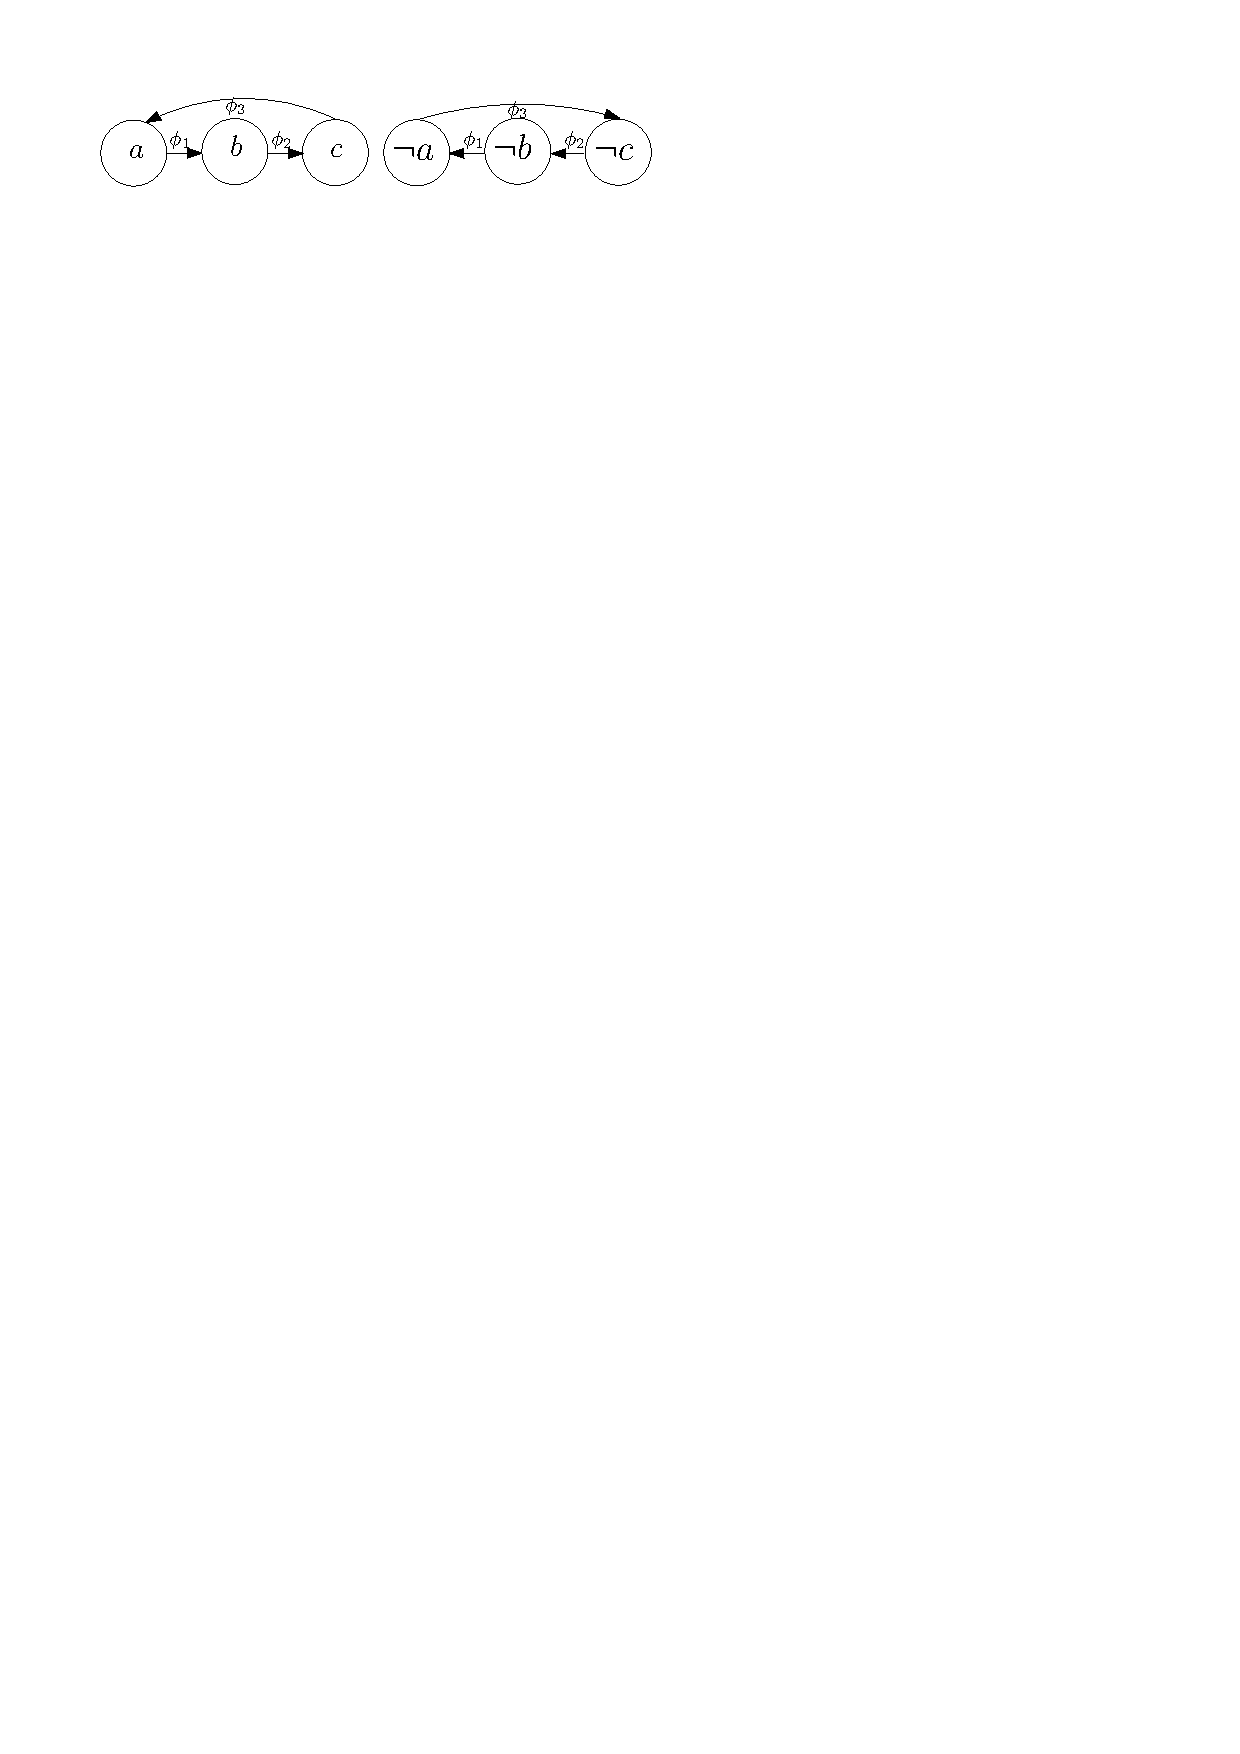
\includegraphics[scale=0.7]{dependency.pdf}
   \caption{Dependency graph of $(a\vee\neg b)\wedge(b\vee\neg c)\wedge(c\vee\neg a)$}
   \label{fig:depend}
\end{figure}

A \emph{path} $\pi$ of a dependency graph $G_\Phi=(V,E)$ is a sequence $l_1...l_n$ of nodes such that for every $i:\ 1\leq i<n$, $(l_i,\phi_i,l_{i+1})\in E$.

A \emph{simple cycle} $c$ of $G_\Phi$ is a path of $G_\Phi$ such that the starting and ending nodes are identical and no repetitions of other nodes.
We use $G_\Phi^{c}$ to denote the set of all the simple cycles of $G_\Phi$.
Given a set of cycles $C\subseteq G_\Phi^c$,
Let $\var(C)$ (resp. $\Lit(C)$ and $E(C)$) denote the set of variables (resp. literals and edges) appeared in $C$,
and $\Phi_{C}$ denote the set of clauses labeled to the edges in $C$.

\begin{proposition}\label{prop:scc-path}
Given a formula $\Phi$ and a set of simple cycles $C\subseteq G_\Phi^{c}$,
if there is no shared edges between each pair of simple cycles in $C$,
then the formula $\Phi_{C}$ is satisfiable. Moveover, for every model $\lambda$ of $\Phi_{C}$,
the assignment $\lambda[\neg \var_{C}]$ is a model $\Phi_C$.
\end{proposition}

\begin{proof}
Consider the assignment $\lambda$ of $\Phi_{C}$ and a cycle $c\in C$, such that for each pair of edges $(l_1,\phi,l_2),(l_1',\phi,l_2')$ of $E(\{c\})$,
$\lambda\models l_1$ iff $\lambda\models l_1'$, and $\lambda\models l_2$ iff $\lambda\models l_2'$.
Then, $\lambda$ is a model of $\Phi_{\{c\}}$. The result immediately follows.
\end{proof}

\begin{lemma}
Given a satisfiable formula $\Phi$ and a set of simple cycles $C\subseteq G_\Phi^{c}$, if $\var(C)\cap \var(\Phi\setminus\Phi_{C})=\emptyset$ or $\Lit(C)\cap \Lit(\Phi\setminus\Phi_C)=\{l\}$, where the literal $l$ is a non-backbone literal for the formula $\Phi\setminus\Phi_C$, then the literals in $\Lit(C)$ are non-backbone literals.
\end{lemma}

\begin{proof}
If $\var(C)\cap \var(\Phi\setminus\Phi_{C})=\emptyset$, then for every $x\in\var(C)$, $\Phi\setminus\Phi_C$ does not contain any
literal of the form $x$ or $\neg x$. Let $\lambda$ be a model of $\Phi$.
By Proposition \ref{prop:scc-path}, $\lambda[\neg\var(C)]\models\Phi_C$.
Therefore, $\lambda[\neg\var_{scc}(\Phi) ]\models\Phi\setminus\Phi_C$.
The result immediately follows.

If $\Lit(C)\cap \Lit(\Phi\setminus\Phi_C)=\{l\}$, where the literal $l$ is a non-backbone literal for the formula $\Phi\setminus\Phi_C$,
there exist two models $\lambda_0$ and $\lambda_1$ of $\Phi$ such that $\lambda_0(x)\neq \lambda_1(x)$.
Let $\lambda_i'$ for $i\in\{0,1\}$ be the assignment such that
for every $y\in\var(C)$, $\lambda_i'(y)=i$, and for every $y'\in \var(\Phi)\setminus\var(C)$,
$\lambda_i'(y')=\lambda_j(y')$ for some $j\in\{0,1\}$ with $\lambda_j(x)=\lambda_i'(x)$.
Obviously, $\lambda_0'$ and $\lambda_1'$ are two models of $\Phi$. Therefore,
the literals in $\Lit(C)$ are non-backbone literals.
\end{proof}

We adapt the algorithm from \cite{Jon75} to identify non-backbone literals from $F(\Phi,\lambda)$ and these non-backbone literals are added in $\NBLap(\Phi)$.
This gives a more tight approximation set of backbone literals which is the desired set $\BLap(\Phi)$.
\fi

\subsection{Computing Parts of Exact Backbone Using Assumptions}

Although WCB Algorithm is able to compute an approximation set of backbone, it still needs at least one SAT testing to determine whether a literal is backbone, which may need a long solving time. Inspired by \cite{JLM15}, we use assumptions in MINISAT as a heuristic strategy to accelerate SAT testing, named Whitening-assumptions-based Algorithm, WAB for short.

Experiments show that given the same formula $\Phi$, SAT testings with assumptions are generally faster then the ones without assumptions. It's because that assumptions help to make the initial decisions of a SAT solving, given an assumption $\gamma$ with k literals in it, it reduces $2^k$ states of the searching spaces. SAT testing with a longer assumptions will return faster.

A formula $\Phi$ is satisfiable with assumption $\gamma$ indicates that there exists a model $\lambda\models\Phi$, such that $\forall l\in\gamma, \lambda(l)=1$. We use $SAT(\Phi,\gamma)$ to denote a SAT testing of $\Phi$ with the assumption of $\gamma$. We use $(b, \lambda, r)$ to denote the result of $SAT(\Phi,\gamma)$. If $b$ is assigned to $1$, a model is returned in $\lambda$, otherwise, a reason of unsatisfiable is returned in $r$. For every literal $l\in\BLap(\Phi)$, $\neg l$ is selected to $\gamma$.
If there is exactly one reason $l_b$ returned from $SAT(\Phi,\gamma)$, it indicates that $\neg l_b$ must be a backbone of $\Phi$.


\begin{algorithm2e}
\SetKwInOut{Input}{Input}
\SetKwInOut{Output}{Output}
\SetAlgoShortEnd
\SetFillComment
\Input{a satisfiable formula $\Phi$ and $\BLap(\Phi)$}
\Output{under-approximation of backbone literals $\BLapu(\Phi)$ }
$\BLapu(\Phi):=\emptyset$\;
$\gamma:=\{l\in\Lit(\Phi) \mid \neg l\in\BLap(\Phi)\}$\; \label{alg4:init}
\Repeat {$\gamma==\emptyset$}{
    $(b, \lambda', r):=SAT(\Phi,\gamma)$\; \label{alg4:test}
    \If {$b==0$}{
        \If {$|r|==1$}{
            $l_b:=r_0$\;
            $\BLapu(\Phi):=\BLapu(\Phi)\cup \{\neg l_b\}$\; \label{alg4:bl}
        }
        $\gamma=\gamma\setminus r$\; \label{alg4:cut}
    }
    \If{$b==1$}{
        $\BLap(\Phi):=\BLap(\Phi)\setminus\gamma$\; \label{alg4:remove}
        $\NBLap(\Phi):=\NBLap(\Phi)\cup\gamma$\;
        break\;
    }
}
\Return $\BLapu(\Phi)$\;
\caption{WAB Algorithm for computing under-approximation of backbone $\BLapu(\Phi)$}
\label{alg:assum}
\end{algorithm2e}

Given a model $\lambda$ and a satisfiable formula $\Phi$. We initialize $\gamma$ with $\BLap(\Phi)$ at Line \ref{alg4:init}. We add $\neg l$ to $\gamma$ for every $l\in\BLap(\Phi)$ to block the known model $\lambda$. At Line \ref{alg4:test}, we compute the result of $SAT(\Phi,\gamma)$. All literals in $\gamma$ will be removed from $\BLap(\Phi)$ at Line \ref{alg4:remove} if $b$ is assigned to $1$. Otherwise, all literals in $r$ are removed from $\gamma$ at Line \ref{alg4:cut}. Once $\gamma$ is empty, the iteration stops. If there is exactly one literal $l_b$ in $r$, $\neg l_b$ must be backbone and added to $\BLapu(\Phi)$ at Line \ref{alg4:bl}.

\begin{theorem}
Given a satisfiable formula $\Phi$ and a set of assumptions $\gamma$, $\neg l_b\in\BL(\Phi)$ if $l_b\in\gamma$ and $l_b$ is the only reason that $\Phi$ is not satisfiable under the assumption of $\gamma$.
\end{theorem}

\begin{proof}
Given a satisfiable formula $\Phi$ and a set of assumptions $\gamma$, suppose literal $l_b$ is the only reason returned $r$ from $SAT(\Phi,\gamma)$, i.e., $\forall l\in r, l=l_b$.
It means that there doesn't exist a model $\lambda\models\Phi$, such that $\lambda(l_b)=1$. Therefore, $\neg l_b$ is a backbone literal of $\Phi$, i.e., $\neg l\in\BL(\Phi)$.
\end{proof}

WAB Algorithm is able to compute the approximation of backbones of the given formula. When the length of unsatisfiable reason is 1, WAB saved solving time when determining if a variable is a backbone. Experiments show that, SAT testings with assumptions are generally finished within 1 second, while original SAT testing may take more than 1 minute.

Compared with the original Whitening Algorithm, the accuracy of Whitening-based Algorithm improved by two heuristic strategies (WCB and WAB) has increased. Missing backbone are added to the approximation through WCB and accurate backbone are confirmed with WAB. With a higher accuracy, backbone computing are guided better with $\BLap(\Phi)$.
